%!TEX root = ../../../memoria.tex

\section{\isomorphicAS \javaScriptNAME : el futuro de las aplicaciones \webINT}\label{cap:justificacion:section:web_app}

Cuando se utiliza un \backendAS corriendo una aplicación \javaNAME, \phpNAME o \railsNAME, el proceso ocurre muy lejos del usuario. Los clientes solicitan datos llamando una \uriNAME. En respuesta, la aplicación trae datos desde una \dataBaseDB, realiza algún procedimiento para crear \htmlNAME y envía los resultados al cliente. Mientras mayor sea el número de clientes que realizan la misma solicitud, los mecanismos inteligentes de \caching pueden ser usados por el \serverAS. \sitesINT de noticias funcionan particularmente bien en este tipo de paradigma.
%When using a backend running a Java, PHP, or Rails application, processing takes place far away from the user. Clients request data by calling a URI. In response the application fetches data from a database, performs some processing to create HTML and sends the results to a client. The more clients request the same information, the more clever caching mechanisms can be used by the server. News sites work particularly well with this paradigm.

En un escenario en donde cada usuario realiza solicitudes para crear vistas altamente individualizadas, un único proceso de instancia rápidamente se convierte en un cuello de botella. Considerando a \facebook como un ejemplo: Dos personas nunca verán exactamente un mismo \facebookwall, esto es calculado individualmente para cada usuario. Esto agrega una gran cantidad de \stress en el servidor mientras el cliente está en su mayoría de tiempo \idle, esperando una respuesta.
%In a scenario where each user has the means to create highly individualized views a single processing instance can quickly become a bottle neck. Consider Facebook as an example: No two people will ever see the exact same wall, it needs to be computed for each user individually. That puts a lot of stress on the servers while clients idle most of the time, waiting for a response.

Cuando el poder de procesamiento de un cliente era relativamente limitado, este enfoque tenia sentido, pero en la actualidad un solo \smartphoneCPT tiene más poder de cómputo que muchos de los súper computadores en los primeros años de la \webINT. Los nuevos enfoques toman ventaja de ese poder y delegan la mayoría del proceso a los clientes. \frontEndsAS inteligentes solicitan información al \serverAS y montan el \htmldomNAME en el \browserINT.
%When the processing power of clients was relatively limited this made perfect sense, but these days a single iPhone already has more computing power than most super computers in the early days of the web. Meteor takes advantage of that power and delegates most of the processing to the clients. Smart front-ends request data from the server and assemble the DOM only in the browser or mobile device (see Figure 1-4).

Este enfoque \clientcentric implica dos ventajas significativas:
%This client-centric approach brings two significant advantages:
\begin{itemize}
	\item Menos necesidad de transferencia de información entre el \serverAS y el cliente, lo que esencialmente se traduce como tiempos de respuesta mas rápidos.
%1. Less data needs to be transferred between server and client which essentially translates into quicker response times
	\item Existe una menor probabilidad de que el procesamiento sea bloqueado por otros usuarios debido a peticiones de duración prolongada, ya que la mayor parte del trabajo se realiza individualmente en cada cliente.
%2. Processing is less likely to be blocked by other users due to long-running requests, as most of the work is done on each individual client
\end{itemize}

La arquitectura \clientserver se basa en \statelessconnectionsINT. clientes solicitan información una vez, el \serverAS responde y la conexión es cerrada nuevamente. Actualizaciones en otros clientes pueden suceder, a menos que explícitamente realiza una solicitud al \serverAS nuevamente, no verán actualizaciones. No existe un canal de \feedback del \serverAS al cliente para enviar actualizaciones de contenido.

Mover el proceso desde un solo \serverAS a múltiples clientes envuelve moverse en dirección a una plataforma de cómputo distribuida. En tal situación, los datos deben ser enviados en ambas direcciones.

Después de muchos años de avance, se desarrollaron soluciones muy creativas que impulsaron a los \browsersINT a mejorar para mantenerse a la par. 
Actualmente la \webINT se ha transformado en una plataforma de aplicaciones \fullyfeatured, \runtimesCPT \javaScriptNAME rápidos y \standard \htmlfive que permite crear aplicaciones que antes eran solo posibles en plataformas nativas.

\subsection{\singlePageAppINT}

No pasó mucho tiempo hasta que los desarrolladores comenzaron a crear aplicaciones completas en el \browserINT utilizando las nuevas capacidades de \javaScriptNAME y \htmlfive para crear \singlePageAppINT. Una \spa es una aplicación \webINT completa, la cual solo tiene una página, que es usada como un contenedor para todas las páginas \webINT de la aplicación y utiliza \javaScriptNAME, \htmlfive y \cssNAME para todas las interacciones \frontEndsAS. En \spas no hay \posts completos de vuelta al \serverAS, no hay refrescos completos de una página \webINT, y no hay objetos embebidos. La principal diferencia con las aplicaciones \webINT tradicionales es la naturaleza de las \requests y \responsesINT que siguen al \requestINT \httpNAME inicial. Con \spa se utiliza \ajaxNAME para \requestINT datos y se obtiene un \responsesINT correspondiente a datos \jsonNAME. Una vez que la información es recibida por el cliente, este hará un despliegue parcial de \htmlNAME para representar los cambios. Incluso, moviéndonos de una página a otra en un \spa ocurre en \clientSideAS, lo que es diferente a lo que sucede en aplicaciones tradicionales y \ria.

Librerías como \backbonejsNAME \emberjsNAME, y \angularjsNAME usualmente son referidas como librerías \clientSideAS \mvcAS o \mvvmAS. La arquitectura típica \clientSideAS \mvcAS se ve similar a la \refFigura{figure:client_side_mvc}. 
%Libraries like Backbone.js, Ember.js, and Angular.js are often referred to as client-side MVC (Model-View-Controller) or MVVM (Model-View-ViewModel) libraries. The typical client-side MVC architecture looks something like this:

% GRAFICO CLIENT SIDE MVC 

%\begin{figure}[h!]
\begin{figure}[H]
	\centering
	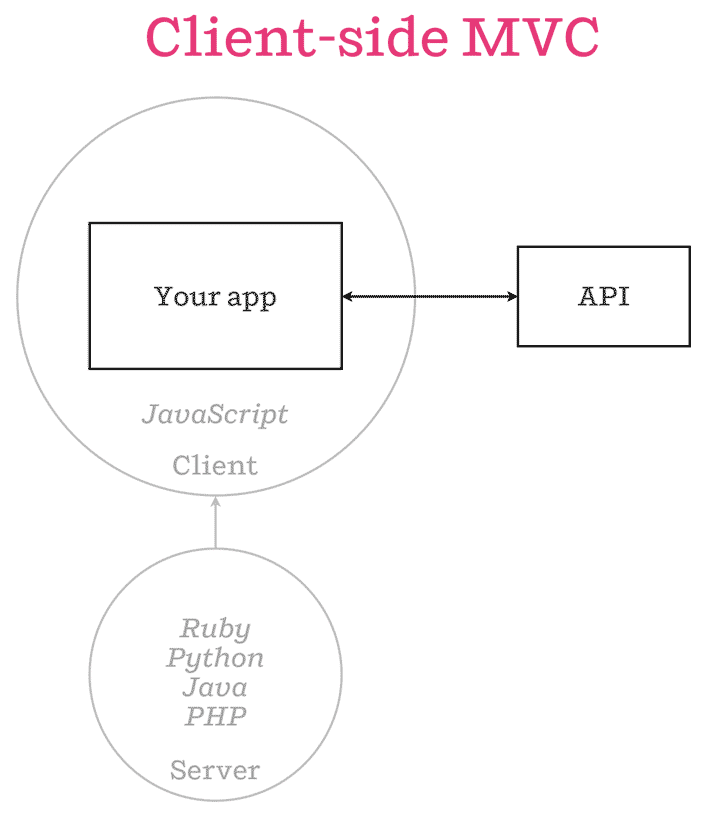
\includegraphics[width=0.5\textwidth]{figuras/estadoArte/isomorphic-client-side-mvc.png}

	\caption{\clientSideAS \mvcAS.}
	\label{figure:client_side_mvc}
\end{figure}

% Definition of circles
% \def\firstcircle{(0,0) circle (2)}
% \def\secondcircle{(0,-5) circle (1)}

% \def\firstrectangle{(-1.5,1) rectangle (1.5,-1)}

% \def\secondrectangle{(4,0.5) rectangle (6.5,-0.5)}

% \colorlet{circle edge}{blue!50}
% \colorlet{circle area}{blue!20}

% \tikzset{filled/.style={fill=circle area, draw=circle edge, thick},
%     outline/.style={draw=circle edge, thick}}

% \setlength{\parskip}{5mm}
% % Set A and B
% \begin{tikzpicture}
%     \begin{scope}
%         \clip \firstcircle;
%         \fill[filled] \secondcircle;
%     \end{scope}

%     \draw \firstrectangle node {$Aplicacion$};
%     \draw \secondrectangle node {$API$};

%     \draw[outline] \firstcircle node {$A$};
%     \draw[outline] \secondcircle node {$B$};
%     \node[anchor=south] at (current bounding box.north) {$A \cap B$};
% \end{tikzpicture}









% \newcommand{\mx}[1]{\mathbf{\bm{#1}}} % Matrix command
% \newcommand{\vc}[1]{\mathbf{\bm{#1}}} % Vector command

% % Define the layers to draw the diagram
% \pgfdeclarelayer{background}
% \pgfdeclarelayer{foreground}
% \pgfsetlayers{background,main,foreground}

% % Define block styles used later

% \tikzstyle{sensor}=[draw, fill=blue!20, text width=5em, 
%     text centered, minimum height=2.5em,drop shadow]
% \tikzstyle{ann} = [above, text width=5em, text centered]
% \tikzstyle{wa} = [sensor, text width=10em, fill=red!20, 
%     minimum height=6em, rounded corners, drop shadow]
% \tikzstyle{sc} = [sensor, text width=13em, fill=red!20, 
%     minimum height=10em, rounded corners, drop shadow]

% % Define distances for bordering
% \def\blockdist{2.3}
% \def\edgedist{2.5}

% \begin{tikzpicture}
%     \node (wa) [wa]  {System Combination};
%     \path (wa.west)+(-3.2,1.5) node (asr1) [sensor] {$ASR_1$};
%     \path (wa.west)+(-3.2,0.5) node (asr2)[sensor] {$ASR_2$};
%     \path (wa.west)+(-3.2,-1.0) node (dots)[ann] {$\vdots$}; 
%     \path (wa.west)+(-3.2,-2.0) node (asr3)[sensor] {$ASR_N$};    
   
%     \path (wa.east)+(\blockdist,0) node (vote) [sensor] {$\theta_0,\theta_1,...,\theta_M$\\Estimated Parameters};

%     \path [draw, ->] (asr1.east) -- node [above] {} 
%         (wa.160) ;
%     \path [draw, ->] (asr2.east) -- node [above] {} 
%         (wa.180);
%     \path [draw, ->] (asr3.east) -- node [above] {} 
%         (wa.200);
%     \path [draw, ->] (wa.east) -- node [above] {} 
%         (vote.west);

               
%     \path (wa.south) +(0,-\blockdist) node (asrs) {System Combination - Training};
  
%     \begin{pgfonlayer}{background}
%         \path (asr1.west |- asr1.north)+(-0.5,0.3) node (a) {};
%         \path (wa.south -| wa.east)+(+0.5,-0.3) node (b) {};
%         \path (vote.east |- asrs.east)+(+0.5,-0.5) node (c) {};
          
%         \path[fill=yellow!20,rounded corners, draw=black!50, dashed]
%             (a) rectangle (c);           
%         \path (asr1.north west)+(-0.2,0.2) node (a) {};
            
%     \end{pgfonlayer}
    
%     % Validation Layer is the same except that there are a set of nodes and links which are added
   

%     \path (wa.south)+(-2.0,-7.5) node (syscomb) [sc] {\textbf{System Combination \\Algorithm}\\Estimated Parameters\\from training};
%     \path (syscomb.west)+(-2.2,1.5) node (asrt1) [sensor] {$ASR_1$};
%     \path (syscomb.west)+(-2.2,0.5) node (asrt2)[sensor] {$ASR_2$};
%     \path (syscomb.west)+(-2.2,-1.0) node (dots)[ann] {$\vdots$}; 
%     \path (syscomb.west)+(-2.2,-2.0) node (asrt3)[sensor] {$ASR_N$};    

%     \path [draw, ->] (asrt1.east) -- node [above] {} 
%         (syscomb.160) ;
%     \path [draw, ->] (asrt2.east) -- node [above] {} 
%         (syscomb.180);
%     \path [draw, ->] (asrt3.east) -- node [above] {} 
%         (syscomb.200);

               
%     \path (wa.south) +(0,-\blockdist) node (sct) {System Combination - Training};
 

%     \path (syscomb.east)+(1.0,0.0) node (bwtn) {};

%     % Note how the single nodes are repeated using for loop
%     \foreach \x in {0,1,...,4} 
%     { 
%         \draw (bwtn.east)+(\x,0) node (asr\x-2)[]{}; 
%         \fill (bwtn.east)+(\x,0) circle (0.1cm); 
%     }
   
%     \path [draw, ->] (syscomb.east) -- node [above] {} 
%         (bwtn.east);
% 	\path [draw, ->] (asr0-2) -- node [above] {@} 
%         (asr1-2);
%     \path [draw, -] (asr1-2) -- node [above] {b} 
%         (asr2-2);
%     \path [draw, -] (asr2-2) -- node [above] {z} 
%         (asr3-2);
%     \path [draw, -] (asr3-2) -- node [above] {} 
%         (asr4-2);

%     \path [draw, ->] (asr0-2) edge[bend  right]  node [below] {@} 
%         (asr1-2);
%     \path [draw, ->] (asr1-2) edge[bend  right]  node [below] {b} 
%         (asr2-2);
%     \path [draw, ->] (asr2-2) edge[bend  right]  node [below] {c} 
%         (asr3-2);
%     \path [draw, ->] (asr4-2) node[]{} (asr4-2)+(1.0,0);

%     \begin{scope}[looseness=1.6]
%         \path [draw, ->] (asr0-2) edge[bend  right=90]  node [below] {a} 
%             (asr1-2);
%         \path [draw, ->] (asr1-2) edge[bend  right=90]  node [below] {b} 
%             (asr2-2);
%         \path [draw, ->] (asr2-2) edge[bend  right=90]  node [below] {c} 
%             (asr3-2);
%     \end{scope}
%     \path (asr3-2.east)+(1.5,0.0) node (bw)[sensor] {Best Word Sequence\\$\arg\max$};    

%     \path [draw, -] (asr1-2.east) node [below] {} 
%         (bw.west);
          
%     \begin{pgfonlayer}{background}
%         \path (asrt1.west)+(-0.5,1.0) node (g) {};
%         \path (bw.east |- syscomb.south)+(0.5,-1.5) node (h) {};
         
%         \path[fill=yellow!20,rounded corners, draw=black!50, dashed]
%             (g) rectangle (h);

%         \path [draw, ->] (vote.south) edge[bend  left=90]  node [below] {Used in validation} 
%             (syscomb.30);            

%     \end{pgfonlayer}
    
%     \path (asr1-2.south) +(-\blockdist,-\blockdist) 
%         node (asrs) {System Combination - Validation};

% \end{tikzpicture}

%The bulk of the application logic (views, templates, controllers, models, internationalization, etc.) lives in the client, and it talks to an API for data. The server could be written in any language, such as Ruby, Python, or Java, and it mostly handles serving up an initial barebones page of HTML. Once the JavaScript files are downloaded by the browser, they are evaluated and the client-side app is initialized, fetching data from the API and rendering the rest of the HTML page.

Otro cambio entre \spa y aplicaciones \webINT tradicionales es el manejo de estados. En \spa, dado que no se abandona o refresca la página \webINT principal se puede persistir el estado en la memoria del \browserINT. Incluso, si se desea guardar el estado de la aplicación en escenarios \offline o cuando los usuarios cierran el \browserINT, se puede utilizar \htmlfive \storage para mantener el estado. Después cuando el usuario regrese a \online, puede regresar al último estado de la aplicación sin involucrar al \serverAS.

Esta arquitectura es genial para los desarrolladores, porque la idealizada \singlePageAppINT tiene una separación de conceptos clara entre el cliente y el \serverAS, promoviendo un hermoso \workflowCPT y previene la necesidad de compartir lógica entre ambos, lo que usualmente es escrito en diferentes lenguajes.
%This is great for the developer because the idealized single-page app has a clear separation of concerns between the client and the server, promoting a nice development workflow and preventing the need to share too much logic between the two, which are often written in different languages.

\subsection{No todo lo que brilla es oro}

En la práctica, sin embargo, hay algunos defectos fatales con este enfoque que impide que sea adecuado para muchos casos de uso.
%Trouble in Paradise
%In practice, however, there are a few fatal flaws with this approach that prevent it from being right for many use cases.


\begin{itemize}
	\item
		\textbf{\seoINT}. Una aplicación que puede solo \runCPT en el \clientSideAS no puede entregar \htmlNAME a los \crawlersINT, lo que implica que el \webINT tendrá un \seoINT mediocre por \defaultCPT. Los \crawlersINT actúan enviando un \requestINT a un \webserverINT e interpretando el resultado; pero si el \serverAS \responseINT una página en blanco, esto no tiene mucho valor. Existen algunas soluciones, pero estas requieren algo de trabajo \cite{online_problems_sing_page_app}.
		%SEO
		%An application that can only run in the client-side cannot serve HTML to crawlers, so it will have poor SEO by default. Web crawlers function by making a request to a web server and interpreting the result; but if the server returns a blank page, it’s not of much value. There are workarounds, but not without jumping through some hoops.
	\item
		\textbf{\performanceQA}. Por la misma razón, si el \serverAS no despliega una página completa de \htmlNAME, en lugar de eso el \clientSideAS espera para que \javaScriptNAME lo realice, los usuarios experimentarán críticos segundos de una página en blanco o un \loadingSpinnerCPT antes de ver el contenido de la página. Hay una abundante cantidad de estudios que muestran los drásticos efectos que un \siteINT lento tienen en los usuarios, y por lo tanto su \revenueQA \cite{online_fastView_web_perfor_opti_accele}. \textbf{\amazonNAME afirma} que cada 100ms que se reduce el \loadTimeCPT de una página aumenta el \revenueQA en 1\% \cite{kohavi2007online} \cite{online_psychology_web_performance}.\textbf{ \twitterNAME invirtió un año y 40 ingenieros} para \rebuildingPL su \siteINT para desplegar en el \serverAS en lugar del cliente, afirmando una mejora x5 en la percepción de \loadingTimeCPT \cite{online_improving_web_performance_twitter}.
		%Performance
		%By the same token, if the server doesn’t render a full page of HTML but instead waits for client-side JavaScript to do so, users will experience a few critical seconds of blank page or loading spinner before seeing the content on the page. There are plenty of studies showing the drastic effect a slow site has on users, and thus revenue. Amazon claims that each 100ms reduction in page load time raises revenue by 1%. Twitter spent a year and 40 engineers rebuilding their site to render on the server instead of the client, claiming a 5x improvement in perceived loading time.
	\item
		\textbf{\maintainabilityQA}. Mientras que en el caso ideal se podría dirigir hacia un linda, y limpia separación de conceptos, inevitablemente algunos \bitsPC de la lógica de la aplicación o de la vista terminen duplicados entre el cliente y el \serverAS, usualmente en diferentes lenguajes. Ejemplos comunes son el formateo de  \datePL y \currencyCPT, validación de formularios, y la \routingLogicAS. Esto hace que \maintenanceQA sea una pesadilla, especialmente para aplicaciones más complejas \cite{online_problems_sing_page_app}.
		%Maintainability
		%While the ideal case can lead to a nice, clean separation of concerns, inevitably some bits of application logic or view logic end up duplicated between client and server, often in different languages. Common examples are date and currency formatting, form validations, and routing logic. This makes maintenance a nightmare, especially for more complex apps.
\end{itemize}

%Some developers, myself included, feel bitten by this approach — it’s often only after having invested the time and effort to build a single-page app that it becomes clear what the drawbacks are.

\subsection{Un enfoque híbrido}

La experiencia muestra que la situación más deseable es un híbrido entre el enfoque clásico y el enfoque moderno: Se desea entregar \htmlNAME \fullyFormedCPT desde el \serverAS para \performanceQA y \seoINT, pero también la \speedQA y \flexibilityQA de la lógica de aplicación de \clientSideAS.
%At the end of the day, we really want a hybrid of the new and old approaches: we want to serve fully-formed HTML from the server for performance and SEO, but we want the speed and flexibility of client-side application logic.

Aplicaciones \isomorphicAS \javaScriptNAME son aquellas en que la aplicación \javaScriptNAME puede \runCPT tanto en \clientSideAS como en \serverSideAS.
%To this end, we’ve been experimenting at Airbnb with “Isomorphic JavaScript” apps, which are JavaScript applications that can run both on the client-side and the server-side.

Una aplicación \isomorphicAS debería verse como se representa en \refFigura{figure:isomorphic_client_server_mvc}.
%An isomorphic app might look like this, dubbed here “Client-server MVC”:

\begin{figure}[H]
	\centering
	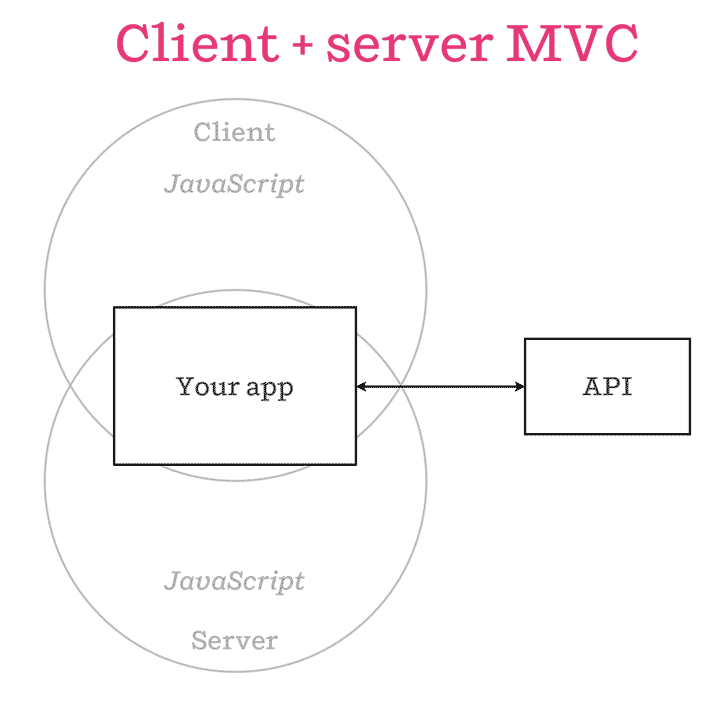
\includegraphics[width=0.5\textwidth]{figuras/estadoArte/isomorphic-client-server-mvc.png}
	\caption{\mvcAS \isomorphicAS  cliente servidor.}
	\label{figure:isomorphic_client_server_mvc}
\end{figure}

Algunas de las aplicaciones y \viewLogicAS que son utilizadas recurrentemente, pueden ser ejecutadas tanto en el \serverAS como en cliente. Esto permite nuevas posibilidades: \performanceQA \optimizationQA, mejor \maintainabilityQA, \seoINT por \defaultCPT, y más  aplicaciones \webINT \statefulINT.
%In this world, some of your application and view logic can be executed on both the server and the client. This opens up all sorts of doors — performance optimizations, better maintainability, SEO-by-default, and more stateful web apps.

Con la aparición de \nodejsNAME, un \fastQA, \stableQA \serverSideAS \javaScriptNAME \runtimeCPT, es factible hacer este sueño realidad. Creando las abstracciones apropiadas, es posible escribir \logicAS de aplicación que corra en el \serverAS y el cliente; justamente la definición de \isomorphicAS \javaScriptNAME.
%With Node.js, a fast, stable server-side JavaScript runtime, we can now make this dream a reality. By creating the appropriate abstractions, we can write our application logic such that it runs on both the server and the client — the definition of isomorphic JavaScript.

\subsection{\isomorphicAS \javaScriptNAME \frameworksPC}
\label{cap:justificacion:subsection:isomorphic_javaScript_framework}

\nodejitsuNAME escribió una gran descripción de una arquitectura \isomorphicAS \javaScriptNAME en 2011 \cite{online_nodejitsu_scaling_iso_js_code}, pero fue adoptado lentamente.
%This idea isn’t new — Nodejitsu wrote a great description of isomorphic JavaScript architecture in 2011 — but it’s been slow to adopt. There have been a few isomorphic frameworks to spring up already.

%Mojito was the first open-source isomorphic framework to get any press. It’s an advanced, full-stack Node.js-based framework, but its dependence on YUI and Yahoo!-specific quirks haven’t led to much popularity in the JavaScript community since they open sourced it in April 2012.

El cliente y el \serverAS son \environmentsPL muy distintos, y por lo tanto es necesario un conjunto de abstracciones que desacoplen la lógica de la aplicación desde su implementación subyacente, así se puede exponer una sola \apiAS para los desarrolladores.
%That these projects tend to be large, full-stack web frameworks speaks to the difficulty of the problem. The client and server are very dissimilar environments, and so we must create a set of abstractions that decouple our application logic from the underlying implementations, so we can expose a single API to the application developer.

\begin{itemize}
	\item
		\textbf{\routingAS}. Se desea un solo \setPL de \routesPC para \mapCPT patrones \uriNAME que \textit{manejar} \routePC. Los \handlersAS de \routePC necesitan disponibilidad de acceso a \httpNAME \headersINT, \cookiesINT, e información \uriNAME, y especificar redireccionamiento sin acceder directamente a \windowLocationINT(\browserINT) o \reqNodeINT y \resNodeINT (\nodejsNAME) \cite{online_isom_js_future_web_apps}.
		%Routing
		%We want a single set of routes that map URI patterns to route handlers. Our route handlers need to be able to access HTTP headers, cookies, and URI information, and specify redirects without directly accessing window.location (browser) or req and res (Node.js).
	\item
		\textbf{\fetchingPC y \persistingPC \dataPC}. Se desea describir los \resourcesCPT necesarios para desplegar una página particular o \componentAS independiente del mecanismo \fetchingPC \cite{online_isom_js_future_web_apps}.
		%El \resDescriptorCPT podría ser simplemente una \uriNAME apuntando a un \apiendpointAS \jsonNAME, o para aplicaciones largas, puede ser útil para \encapsulatePL \resourcesCPT en \modelsAS 
		%Fetching and persisting data
		%We want to describe the resources needed to render a particular page or component independently from the fetching mechanism. The resource descriptor could be a simple URI pointing to a JSON endpoint, or for larger applications, it may be useful to encapsulate resources in models and collections and specify a model class and primary key, which at some point would get translated to a URI.
	\item
		\textbf{\viewRenderingAS}. Ya sea que se decida manipular directamente \htmldomNAME, seguir con un \templatingAS \htmlNAME \stringBasePL, o bien optar como una de las \componentsAS \uiSiglaAS con una abstracción \htmldomNAME, es necesaria la capacidad de generar \markupPL \isomorphicallyAS. Es necesaria la factibilidad de desplegar cualquier \viewAS desde el \serverAS o el cliente, dependiendo solo de las necesidades de la aplicación \cite{online_isom_js_future_web_apps}.
		%View rendering
		%Whether we choose to directly manipulate the DOM, stick with string-based HTML templating, or opt for a UI component library with a DOM abstraction, we need to be able to generate markup isomorphically. We should be able to render any view on either the server or the client, dependent on the needs of our application.
	\item
		\textbf{\buildingPL y \packagingCPT}. Escribir código de aplicaciones \isomorphicAS es la mitad de la batalla. Herramientas como \grunttoolNAME y \browserifyNAME son partes esenciales del \workflowCPT para obtener una aplicación corriendo. Puede existir un número de \buildStepsPL: \compilingPL \templatesAS, incluyendo dependencias \clientSideAS, aplicando transformaciones, \minificationPL, etc. El caso sencillo es combinar todo el código de la aplicación, \viewsAS y \templatesAS en un único \bundleCPT, para aplicaciones grandes, esto puede resultar en cientos de \kilobytesPC para \downloadCPT. Un enfoque más avanzado es crear \dynamicBundlesCPT e introducir \lazyLoadingCPT \assetsAS, sin embargo, esto rápidamente se torna complicado. Herramientas \statAnalyCPT como \esprimaNAME permiten a desarrolladores ambiciosos intentar \optimizationQA y \metaprogrammingPC para reducir \boilerplateCodeAS.
		%Building and packaging
		%It turns out writing isomorphic application code is only half the battle. Tools like Grunt and Browserify are essential parts of the workflow to actually get the app up and running. There can be a number of build steps: compiling templates, including client-side dependencies, applying transforms, minification, etc. The simple case is to combine all application code, views and templates into a single bundle, but for larger apps, this can result in hundreds of kilobytes to download. A more advanced approach is to create dynamic bundles and introduce asset lazy-loading, however this quickly gets complicated. Static-analysis tools like Esprima can allow ambitious developers to attempt advanced optimization and metaprogramming to reduce boilerplate code.
\end{itemize}

Todo \frameworkPC que resuelve estos problemas al mismo tiempo es considerado un \isomorphicJSFwASref. Lo interesante de esto es que este tipo de \frameworksPC \textbf{permite a los desarrolladores enfocarse en la \businessLogicAS}.



